\documentclass[11pt, letterpaper]{article}

\usepackage{listings} % listing package allows us to insert code
\usepackage{upquote}  % upquote package helps to display stata symbols (such as ` ‘ ) correctly
\usepackage{tcolorbox} 

\lstset{
    framerule=1pt,
    frame=tb,
    emphstyle={\small\ttfamily\bfseries\color{Orange}},
    numbers=left,
    numberstyle= \tiny\color{black},
    basicstyle = \small\ttfamily,
    keywordstyle    = \bfseries\color{BrickRed},
    identifierstyle = \bfseries\color{black},
    stringstyle     = \bfseries\color{ForestGreen},
    commentstyle    = \bfseries\color{Violet},
    breaklines      =   true,
    columns         =   fixed,
    basewidth       =   .5em,
    backgroundcolor = \color{white},
    tabsize=2,
    showspaces=false,
    showstringspaces=false,
}


\title{Homework 2: R Practice}
\author{XIANG-JYUN JHANG b08303024 \\ YI-JIE WU b08302129}

\begin{document}

\maketitle


%\assignmentTitle{Your Name}{Your Student Id}{}{}{Homework 1: Stata Practice}

\section{Read Data}


\subsection*{Question 1.1}

The dataset we use comes from Taiwan Education Panel Survey (TEPS) and the Taiwan Education Panel Survey and Beyond (TEPS-B).
It's a broad panel data following three group of students born in 1984-1985 and 1988-1989, doing survey in their junior and high school period and recording their background and performance.  
In the TEPS-B, researchers further tracking the information after those students entering labour market.  We utilize the students' family background and labour market performance to conduct our analysis. 
\\
\\
Since the previous homework helps us to clean the data from the original survey with stata, in this homework, we'll use the cleaned data which includes students' characteristics from high school period survey, and their following performance in 2009 and 2015. Moreover, in order to make code easy to show in code blocks, we only use samples who born in 1984-1985 in this homework, while our real analysis will go through the whole samples.


\subsection*{Question 1.2}

we use the following code to read our working dataset:

\begin{lstlisting}
    library(haven)
    SH_divorce <- read_dta("SH_divorce_outcome2009_outcome2015.dta")
\end{lstlisting}


\subsection*{Question 1.3}

The sample size is 19051, and there're 20 variables in total.

\begin{lstlisting}
    summary.data.frame(SH_divorce)
\end{lstlisting}




\section{Examine Data}


\subsection*{Question 2.1}

The sample size is 19051, and there're 20 variables in total.

\begin{lstlisting}
    summary.data.frame(SH_divorce)
\end{lstlisting}



\section{Create Sample For Analysis}


\subsection*{Question 3.1}

We consider whether the variable $\textit{divorce}$ may have some impact on students' future performance.
The dependent variables are $\textit{University, Public}$, \\
$\textit{Wagelevel, Workyear}$. \\

In the main analysis in our final project, we'll try to control lots of variables from their school period as much as possible, so that we can identify the causal effect of divorce.


\subsection*{Question 3.2}

We create the variable $\textit{priv}\_\textit{cap}$ to specify students who lived in capital city and also studied in private high school.
We believe that students who satisfied this condition are richer than who didn't.

\begin{lstlisting}
    SH_divorce <- mutate(SH_divorce, priv_cap = hs_private * hs_capital)
\end{lstlisting}


\subsection*{Question 3.3}

We use the variable $\textit{hs}\_\textit{capital}, \textit{divorce}$ to categorize the group into 4 subgroups, and see whether the mean between groups are quite different.
The code is in below:

\begin{lstlisting}
    divorce_sum <- summarize(group_by(SH_divorce, divorce, hs_capital), \\
    average_year = mean(work_year_2009,na.rm = TRUE), \\
    average_wage = mean(wage_level_2009,na.rm = TRUE))
\end{lstlisting}

And the results is like
\begin{center}
    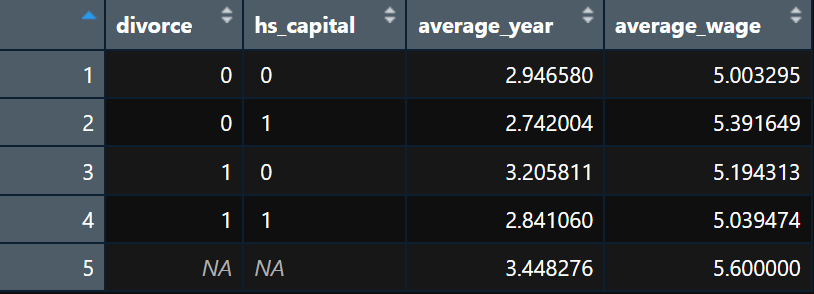
\includegraphics[height=1in]{divorce_sum.png}
\end{center}


\subsection*{Question 3.4}

With the dataset created above, we can merge it into our main dataset.

\begin{lstlisting}
    SH_divorce_1 <- full_join(SH_divorce ,divorce_sum , by = c("hs_capital", "divorce"))
\end{lstlisting}



\section{Visualize Data}

\subsection*{Question 4.1}

Using the dataset created in 3.3, we divide samples into two groups: students who didn't suffer from parents divorce and those who did.
Plot their average working year and average wage in 2009. 

\begin{lstlisting}
    univ_graph <- ggplot(data = SH_divorce_1, aes(x = divorce, y = university)) + geom_bar(stat = "summary", fun = "mean", width = 0.3)
    univ_graph
    ggsave("univ_graph.png", width=3.25,height =3.25)

    workyear_graph <- ggplot(data = SH_divorce_1, aes(x = divorce, y = average_year)) + geom_bar(stat = "summary", fun = "mean", width = 0.3)
    workyear_graph
    ggsave("workyear_graph.png", width=3.25,height =3.25)

    wagelevel_graph <- ggplot(data = SH_divorce_1, aes(x = divorce, y = average_wage)) + geom_bar(stat = "summary", fun = "mean", width = 0.3)
    wagelevel_graph
    ggsave("wagelevel_graph.png", width=3.25,height =3.25)

\end{lstlisting}

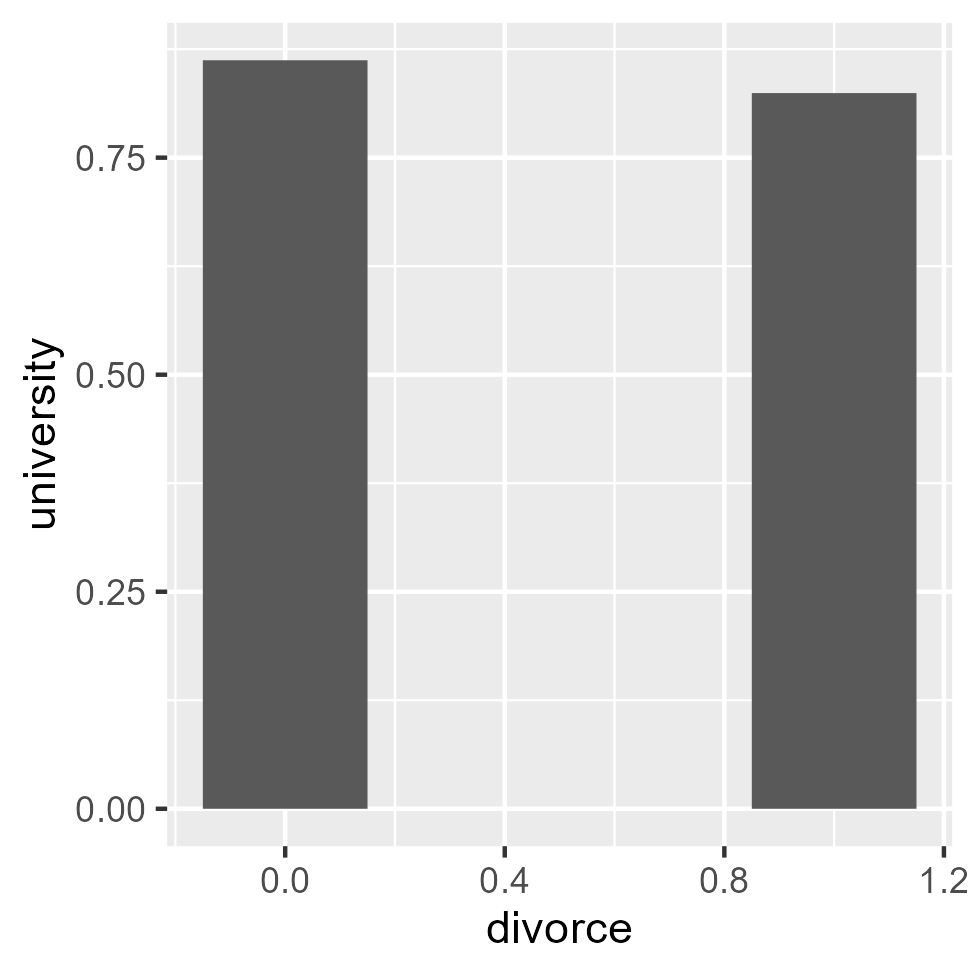
\includegraphics[height=3in]{univ_graph.png} 
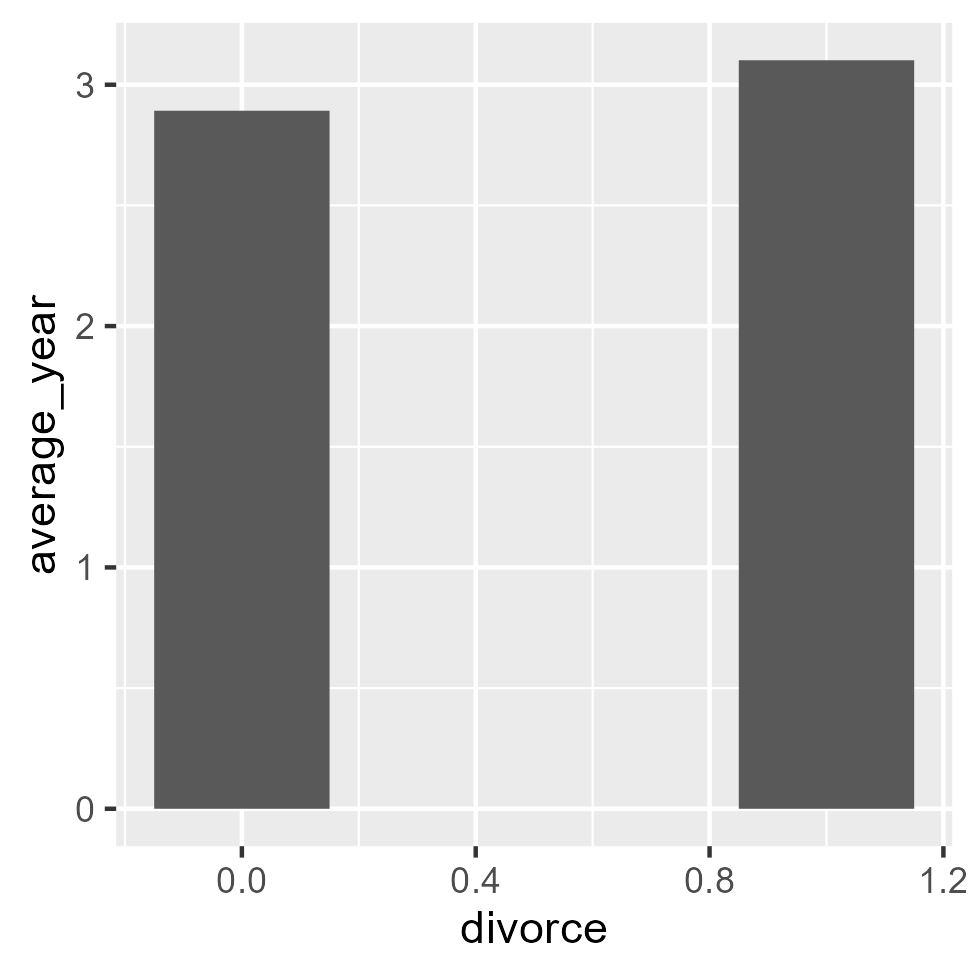
\includegraphics[height=3in]{workyear_graph.png}

\begin{center}    
    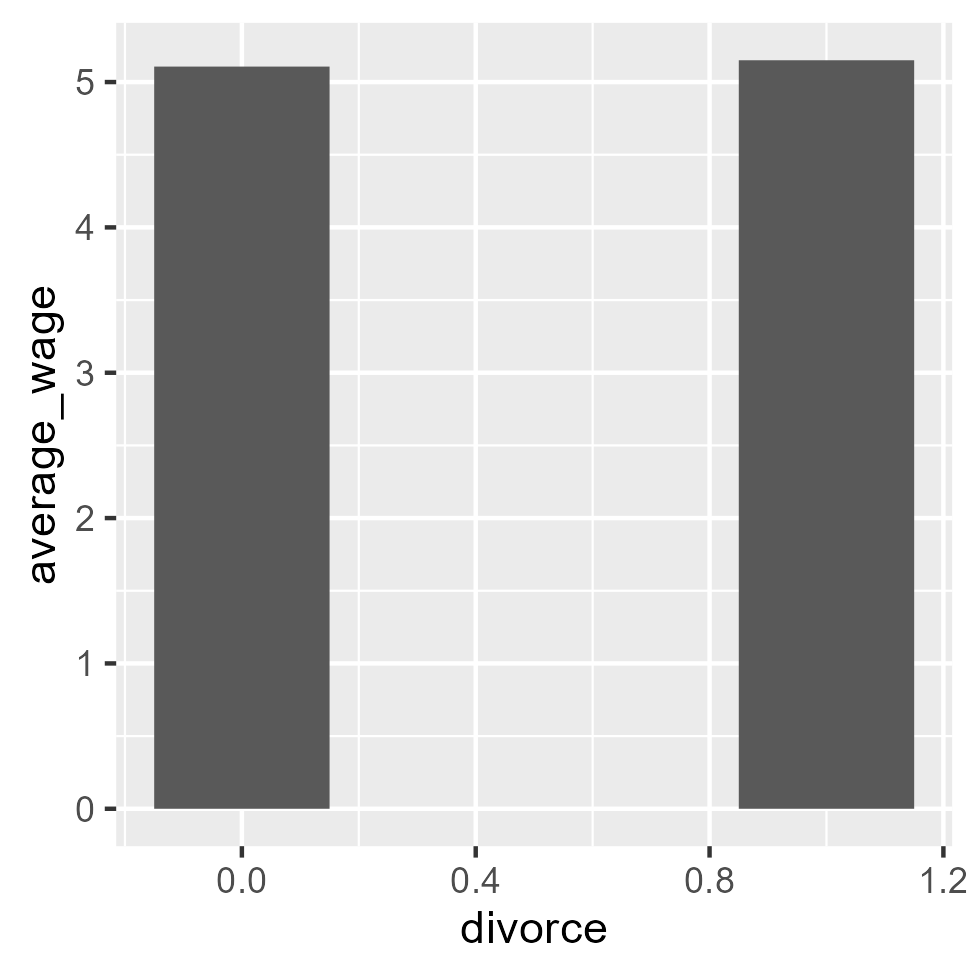
\includegraphics[height=3in]{wagelevel_graph.png}
\end{center}

\subsection*{Question 4.2}

For the university variable, it suggests small different between divorce and non-divorce group. Students in divorce group have less probability to join the university.
For the working year variable, we see the quite different pattern between two groups. It is possible that students in divorce groups are forced to work earlier so that they can support their single parents in economic level.
However, wage lavels are not quite different, the reason may be that freshmen in labor market always get lower payment since they don't have much experience.

\section{Prelimilary Analysis}

\subsection*{Question 5.1}

Since there might be some factos that also influence $\textit{divorce}$ and our dependent variables, we need to add variables as much as possible so that there is no omitted variable problem.
Luckily, we have much information about students' situation in their school period. Thus, we try to include all the possible control variables and use PDS method to help us choose the good control variables.
In this way, we hope that we can overcome the problem and make proper estimations.

The model is as following:
\[
Y_i = \beta_0 + \beta_1 D_i + \bigcup_{j \in A \cup B} \pi_j W_i^j + \epsilon_i
\]
where A and B are the variables choosed in first and second stage.


\subsection*{Question 5.2}

In our topic, we use PDS method to avoid the omitted variable problem, and also verify that our estimation is the causal effect.
We use four dependent variables: University, Public, Wagelevel2009, WorkYear2009, which enable us to understand the difference effect of divorce. 

\begin{lstlisting}
    pdslasso <- read_dta("SH_pds.dta")

    y1 = pdslasso[, 14]
    y2 = pdslasso[, 15, drop = F]
    y3 = pdslasso[, 17, drop = F]
    y4 = pdslasso[, 19, drop = F]
    
    d = pdslasso[, 5]
    X = data.matrix(pdslasso[, -c(1, 5,6,14:20)])
    varnames = colnames(pdslasso)
    
    university_pds <- rlassoEffect(X, y1, d, method = "double selection")
    summary(university_pds)
    
    
    public_pds <- rlassoEffect(X, y2, d, method = "double selection")
    summary(public_pds)
    
    wage2009_pds <- rlassoEffect(X, y3, d, method = "double selection")
    summary(wage2009_pds)
    
    work2009_pds <- rlassoEffect(X, y4, d, method = "double selection")
    summary(work2009_pds)

\end{lstlisting}

\subsection*{Question 5.3}

The coefficient is only significant in university and work2009.
First, the coeffecient is -0.02 when the dependent variable is University, which means that divorce only make 2 percent decrease in the probability of studing university.
Given that the University has mean 0.86 and variance 0.35, the effect of divorce is not really severe. 
Second, the coeffecient is 0.21. It suggests that students in divorce family tend to join the labor market earlier than peers. \\

However, this is only the preliminary result.
In the main analysis in our final project, we will analyze CP groups(born in 1988-1989) estimators and try digging into the group differences. 

\end{document}
